\documentclass{article}
\usepackage {nopageno}
\usepackage{caption}
\usepackage{subcaption}
\usepackage{tikz}
\usetikzlibrary{bayesnet}
\usepackage{graphicx}
\usepackage{fontspec}
\usepackage{multicol}
\usepackage{mathtools}
\usepackage{amssymb}

% Expectation operator
\DeclareMathOperator*{\E}{\mathbb{E}}

\begin{document}
    \title{Trump's Top 10,000 Tweets Since He Started Running for President, by Retweet (WIP)}
    \author{Matthew Woods (mattwoods243@outlook.com)}
    \maketitle
    
    % Pearson's correlation coefficient: see wikipedia.com
    %     https://en.wikipedia.org/wiki/Pearson_correlation_coefficient#Definition
    %     See Expectation Operator (Expected Value): https://en.wikipedia.org/wiki/Expected_value
    \begin{flalign}
        \rho_{X, Y} &= \frac{\E{[XY]} - \E{[X]}\E{[Y]}}{\sqrt{\E{[X^{2}]} - (\E{[X]})^{2}} \sqrt{\E{[Y^{2}]}- (\E{[Y]})^{2}}} \\
                    &= \frac{\E{[(X - \mu_X)(Y - \mu_Y)]}}{\sigma_X \sigma_Y} \\
                    &= \frac{cov(X, Y)}{\sigma_X \sigma_Y}
    \end{flalign}
    
    \begin{figure}
         \hspace{-1.5cm}
         \begin{tikzpicture}
\node[const] (isLie) [xshift=5.500000000000000cm, yshift=0.000000000000000cm, minimum size=1.5cm] {isLie}; \node[const] (isMisspeaking) [xshift=5.400607834944886cm, yshift=1.040881843982256cm, minimum size=1.5cm] {isMisspeaking}; \node[const] (isCantBeThatDumb) [xshift=5.106023631588400cm, yshift=2.044143506131801cm, minimum size=1.5cm] {isCantBeThatDumb}; \node[const] (isOpposite) [xshift=4.626894430571497cm, yshift=2.973524496005786cm, minimum size=1.5cm] {isOpposite}; \node[const] (isInsinuating) [xshift=3.980537209577886cm, yshift=3.795434563151616cm, minimum size=1.5cm] {isInsinuating}; \node[const] (isPreemptive) [xshift=3.190313002641591cm, yshift=4.480167736276846cm, minimum size=1.5cm] {isPreemptive}; \node[const] (isElection) [xshift=2.284782571510375cm, yshift=5.002975974449851cm, minimum size=1.5cm] {isElection}; \node[const] (isIKnowYouAreButWhatAmI) [xshift=1.296674145301850cm, yshift=5.344963625779479cm, minimum size=1.5cm] {isIKnowYouAreButWhatAmI}; \node[const] (isRacist) [xshift=0.261700537030583cm, yshift=5.493770365506544cm, minimum size=1.5cm] {isRacist}; \node[const] (isHitler) [xshift=-0.782731610503067cm, yshift=5.444017930345130cm, minimum size=1.5cm] {isHitler}; \node[const] (isRussia) [xshift=-1.798873798245818cm, yshift=5.197504502930677cm, minimum size=1.5cm] {isRussia}; \node[const] (isUkraine) [xshift=-2.749999999999999cm, yshift=4.763139720814413cm, minimum size=1.5cm] {isUkraine}; \node[const] (isChina) [xshift=-3.601734036699067cm, yshift=4.156622658948421cm, minimum size=1.5cm] {isChina}; \node[const] (isIran) [xshift=-4.323292021085330cm, yshift=3.399874424213330cm, minimum size=1.5cm] {isIran}; \node[const] (isNukes) [xshift=-4.888594967602079cm, yshift=2.520245869500758cm, minimum size=1.5cm] {isNukes}; \node[const] (isExecutivePrivilege) [xshift=-5.277211354879735cm, yshift=1.549529062627865cm, minimum size=1.5cm] {isExecutivePrivilege}; \node[const] (isSmear) [xshift=-5.475095574151966cm, yshift=0.522808238173006cm, minimum size=1.5cm] {isSmear}; \node[const] (isSexist) [xshift=-5.475095574151966cm, yshift=-0.522808238173004cm, minimum size=1.5cm] {isSexist}; \node[const] (isCelebrity) [xshift=-5.277211354879736cm, yshift=-1.549529062627862cm, minimum size=1.5cm] {isCelebrity}; \node[const] (isPentagon) [xshift=-4.888594967602079cm, yshift=-2.520245869500757cm, minimum size=1.5cm] {isPentagon}; \node[const] (isNickname) [xshift=-4.323292021085333cm, yshift=-3.399874424213327cm, minimum size=1.5cm] {isNickname}; \node[const] (isXenophobic) [xshift=-3.601734036699069cm, yshift=-4.156622658948420cm, minimum size=1.5cm] {isXenophobic}; \node[const] (isMAGA) [xshift=-2.750000000000003cm, yshift=-4.763139720814412cm, minimum size=1.5cm] {isMAGA}; \node[const] (isReligious) [xshift=-1.798873798245820cm, yshift=-5.197504502930676cm, minimum size=1.5cm] {isReligious}; \node[const] (isPandemic) [xshift=-0.782731610503069cm, yshift=-5.444017930345129cm, minimum size=1.5cm] {isPandemic}; \node[const] (isAllCaps) [xshift=0.261700537030583cm, yshift=-5.493770365506544cm, minimum size=1.5cm] {isAllCaps}; \node[const] (isRINO) [xshift=1.296674145301846cm, yshift=-5.344963625779481cm, minimum size=1.5cm] {isRINO}; \node[const] (isFirstImpeachment) [xshift=2.284782571510373cm, yshift=-5.002975974449852cm, minimum size=1.5cm] {isFirstImpeachment}; \node[const] (isSecondImpeachment) [xshift=3.190313002641588cm, yshift=-4.480167736276847cm, minimum size=1.5cm] {isSecondImpeachment}; \node[const] (isSoTrue) [xshift=3.980537209577886cm, yshift=-3.795434563151616cm, minimum size=1.5cm] {isSoTrue}; \node[const] (isInTwoWeeks) [xshift=4.626894430571494cm, yshift=-2.973524496005790cm, minimum size=1.5cm] {isInTwoWeeks}; \node[const] (isWitchHunt) [xshift=5.106023631588398cm, yshift=-2.044143506131805cm, minimum size=1.5cm] {isWitchHunt}; \node[const] (isAntifa) [xshift=5.400607834944886cm, yshift=-1.040881843982258cm, minimum size=1.5cm] {isAntifa}; \node[const] (7) [xshift=6.500000000000000cm, yshift=0.000000000000000cm, minimum size=1.5cm] {7}; \node[const] (491) [xshift=6.382536532207594cm, yshift=1.230133088342666cm, minimum size=1.5cm] {491}; \node[const] (496) [xshift=6.034391564604473cm, yshift=2.415805961792129cm, minimum size=1.5cm] {496}; \node[const] (68) [xshift=5.468147963402678cm, yshift=3.514165313461384cm, minimum size=1.5cm] {68}; \node[const] (220) [xshift=4.704271247682956cm, yshift=4.485513574633727cm, minimum size=1.5cm] {220}; \node[const] (1) [xshift=3.770369912212788cm, yshift=5.294743688327181cm, minimum size=1.5cm] {1}; \node[const] (8) [xshift=2.700197584512262cm, yshift=5.912607969804369cm, minimum size=1.5cm] {8}; \node[const] (197) [xshift=1.532433080811277cm, yshift=6.316775194103021cm, minimum size=1.5cm] {197}; \node[const] (4) [xshift=0.309282452854326cm, yshift=6.492637704689551cm, minimum size=1.5cm] {4}; \node[const] (7) [xshift=-0.925046448776353cm, yshift=6.433839372226063cm, minimum size=1.5cm] {7}; \node[const] (186) [xshift=-2.125941761563239cm, yshift=6.142505321645346cm, minimum size=1.5cm] {186}; \node[const] (4) [xshift=-3.249999999999999cm, yshift=5.629165124598852cm, minimum size=1.5cm] {4}; \node[const] (1) [xshift=-4.256594770644353cm, yshift=4.912372233302679cm, minimum size=1.5cm] {1}; \node[const] (14) [xshift=-5.109345115828117cm, yshift=4.018033410433936cm, minimum size=1.5cm] {14}; \node[const] (1) [xshift=-5.777430416257002cm, yshift=2.978472391228169cm, minimum size=1.5cm] {1}; \node[const] (122) [xshift=-6.236704328494232cm, yshift=1.831261619469295cm, minimum size=1.5cm] {122}; \node[const] (8) [xshift=-6.470567496725049cm, yshift=0.617864281477189cm, minimum size=1.5cm] {8}; \node[const] (22) [xshift=-6.470567496725049cm, yshift=-0.617864281477187cm, minimum size=1.5cm] {22}; \node[const] (49) [xshift=-6.236704328494234cm, yshift=-1.831261619469291cm, minimum size=1.5cm] {49}; \node[const] (19) [xshift=-5.777430416257003cm, yshift=-2.978472391228167cm, minimum size=1.5cm] {19}; \node[const] (46) [xshift=-5.109345115828120cm, yshift=-4.018033410433932cm, minimum size=1.5cm] {46}; \node[const] (42) [xshift=-4.256594770644353cm, yshift=-4.912372233302678cm, minimum size=1.5cm] {42}; \node[const] (5) [xshift=-3.250000000000003cm, yshift=-5.629165124598850cm, minimum size=1.5cm] {5}; \node[const] (2) [xshift=-2.125941761563242cm, yshift=-6.142505321645344cm, minimum size=1.5cm] {2}; \node[const] (7) [xshift=-0.925046448776354cm, yshift=-6.433839372226062cm, minimum size=1.5cm] {7}; \node[const] (3) [xshift=0.309282452854325cm, yshift=-6.492637704689551cm, minimum size=1.5cm] {3}; \node[const] (33) [xshift=1.532433080811273cm, yshift=-6.316775194103022cm, minimum size=1.5cm] {33}; \node[const] (153) [xshift=2.700197584512259cm, yshift=-5.912607969804371cm, minimum size=1.5cm] {153}; \node[const] (4) [xshift=3.770369912212787cm, yshift=-5.294743688327183cm, minimum size=1.5cm] {4}; \node[const] (4) [xshift=4.704271247682955cm, yshift=-4.485513574633728cm, minimum size=1.5cm] {4}; \node[const] (7) [xshift=5.468147963402675cm, yshift=-3.514165313461389cm, minimum size=1.5cm] {7}; \node[const] (5) [xshift=6.034391564604470cm, yshift=-2.415805961792132cm, minimum size=1.5cm] {5}; \node[const] (220) [xshift=6.382536532207593cm, yshift=-1.230133088342669cm, minimum size=1.5cm] {220}; \edge [-, color=red!20.034052224863295!white, line width=0.400681044497266pt] {favorites} {isDeleted}; \edge [-, color=blue!73.38805042537888!white, line width=1.467761008507578pt] {retweets} {favorites}; \edge [-, color=red!4.768998241476276!white, line width=0.095379964829526pt] {isFlagged} {isDeleted}; \edge [-, color=red!10.67065510815717!white, line width=0.213413102163143pt] {isLie} {isDeleted}; \edge [-, color=red!9.694392234324695!white, line width=0.193887844686494pt] {isLie} {retweets}; \edge [-, color=blue!38.90790064832985!white, line width=0.778158012966597pt] {isLie} {isFlagged}; \edge [-, color=red!1.5318973783930332!white, line width=0.030637947567861pt] {isPreemptive} {isDeleted}; \edge [-, color=blue!7.942358486583891!white, line width=0.158847169731678pt] {isPreemptive} {isLie}; \edge [-, color=red!9.711629582981372!white, line width=0.194232591659627pt] {isElection} {isDeleted}; \edge [-, color=blue!45.51222286900394!white, line width=0.910244457380079pt] {isElection} {isFlagged}; \edge [-, color=blue!72.15875553426622!white, line width=1.443175110685324pt] {isElection} {isLie}; \edge [-, color=blue!9.232183413918671!white, line width=0.184643668278373pt] {isElection} {isPreemptive}; \edge [-, color=red!1.0788027248458196!white, line width=0.021576054496916pt] {isIKnowYouAreButWhatAmI} {isDeleted}; \edge [-, color=red!6.818744387282318!white, line width=0.136374887745646pt] {isIKnowYouAreButWhatAmI} {favorites}; \edge [-, color=red!5.213750061675352!white, line width=0.104275001233507pt] {isIKnowYouAreButWhatAmI} {retweets}; \edge [-, color=red!3.594016082243194!white, line width=0.071880321644864pt] {isIKnowYouAreButWhatAmI} {isFlagged}; \edge [-, color=red!1.1544696675305315!white, line width=0.023089393350611pt] {isIKnowYouAreButWhatAmI} {isPreemptive}; \edge [-, color=red!1.431492842535793!white, line width=0.028629856850716pt] {isRacist} {isDeleted}; \edge [-, color=red!3.6877150918707087!white, line width=0.073754301837414pt] {isRacist} {retweets}; \edge [-, color=red!4.76899824147629!white, line width=0.095379964829526pt] {isRacist} {isFlagged}; \edge [-, color=red!7.224474007983909!white, line width=0.144489480159678pt] {isRacist} {isLie}; \edge [-, color=red!1.5318973783930478!white, line width=0.030637947567861pt] {isRacist} {isPreemptive}; \edge [-, color=red!1.0788027248458252!white, line width=0.021576054496917pt] {isRacist} {isIKnowYouAreButWhatAmI}; \edge [-, color=red!8.945591997176!white, line width=0.178911839943520pt] {isHitler} {isDeleted}; \edge [-, color=red!9.213594725687695!white, line width=0.184271894513754pt] {isHitler} {retweets}; \edge [-, color=blue!41.179151150670364!white, line width=0.823583023013407pt] {isHitler} {isFlagged}; \edge [-, color=blue!65.60806262792738!white, line width=1.312161252558548pt] {isHitler} {isLie}; \edge [-, color=blue!67.94458653183128!white, line width=1.358891730636625pt] {isHitler} {isElection}; \edge [-, color=red!1.078802724845805!white, line width=0.021576054496916pt] {isRussia} {isDeleted}; \edge [-, color=red!3.5940160822432494!white, line width=0.071880321644865pt] {isRussia} {isFlagged}; \edge [-, color=red!1.1544696675305384!white, line width=0.023089393350611pt] {isRussia} {isPreemptive}; \edge [-, color=red!1.0788027248458232!white, line width=0.021576054496916pt] {isRussia} {isRacist}; \edge [-, color=red!2.039083869808268!white, line width=0.040781677396165pt] {isIran} {isDeleted}; \edge [-, color=red!6.7931791905519905!white, line width=0.135863583811040pt] {isIran} {isFlagged}; \edge [-, color=red!15.199769125486467!white, line width=0.303995382509729pt] {isIran} {isLie}; \edge [-, color=red!13.833689309358194!white, line width=0.276673786187164pt] {isIran} {isElection}; \edge [-, color=red!1.53669593697834!white, line width=0.030733918739567pt] {isIran} {isIKnowYouAreButWhatAmI}; \edge [-, color=red!2.039083869808268!white, line width=0.040781677396165pt] {isIran} {isRacist}; \edge [-, color=red!12.742510339775926!white, line width=0.254850206795519pt] {isIran} {isHitler}; \edge [-, color=red!1.5366959369783266!white, line width=0.030733918739567pt] {isIran} {isRussia}; \edge [-, color=red!6.833429287410087!white, line width=0.136668585748202pt] {isSmear} {isDeleted}; \edge [-, color=red!10.005036934509029!white, line width=0.200100738690181pt] {isSmear} {favorites}; \edge [-, color=red!9.450325966401554!white, line width=0.189006519328031pt] {isSmear} {retweets}; \edge [-, color=blue!9.377338633750082!white, line width=0.187546772675002pt] {isSmear} {isLie}; \edge [-, color=blue!15.787135265062666!white, line width=0.315742705301253pt] {isSmear} {isIKnowYouAreButWhatAmI}; \edge [-, color=red!6.833429287410066!white, line width=0.136668585748201pt] {isSmear} {isRacist}; \edge [-, color=red!9.73384918275266!white, line width=0.194676983655053pt] {isSmear} {isIran}; \edge [-, color=red!1.5318973783930292!white, line width=0.030637947567861pt] {isCelebrity} {isDeleted}; \edge [-, color=red!5.103494538427082!white, line width=0.102069890768542pt] {isCelebrity} {isFlagged}; \edge [-, color=red!11.419092083594656!white, line width=0.228381841671893pt] {isCelebrity} {isLie}; \edge [-, color=red!1.6393442622951087!white, line width=0.032786885245902pt] {isCelebrity} {isPreemptive}; \edge [-, color=red!10.39280075738252!white, line width=0.207856015147650pt] {isCelebrity} {isElection}; \edge [-, color=red!1.1544696675305361!white, line width=0.023089393350611pt] {isCelebrity} {isIKnowYouAreButWhatAmI}; \edge [-, color=red!6.544829021709947!white, line width=0.130896580434199pt] {isCelebrity} {isHitler}; \edge [-, color=red!1.1544696675305424!white, line width=0.023089393350611pt] {isCelebrity} {isRussia}; \edge [-, color=red!2.182104682374406!white, line width=0.043642093647488pt] {isCelebrity} {isIran}; \edge [-, color=red!2.5776073414517877!white, line width=0.051552146829036pt] {isPentagon} {isDeleted}; \edge [-, color=red!5.740148763975768!white, line width=0.114802975279515pt] {isPentagon} {isFlagged}; \edge [-, color=red!13.290758385258282!white, line width=0.265815167705166pt] {isPentagon} {isLie}; \edge [-, color=red!13.484573880202797!white, line width=0.269691477604056pt] {isPentagon} {isElection}; \edge [-, color=red!1.9425384053020787!white, line width=0.038850768106042pt] {isPentagon} {isIKnowYouAreButWhatAmI}; \edge [-, color=red!2.577607341451799!white, line width=0.051552146829036pt] {isPentagon} {isRacist}; \edge [-, color=red!1.942538405302081!white, line width=0.038850768106042pt] {isPentagon} {isRussia}; \edge [-, color=blue!55.4563979943792!white, line width=1.109127959887584pt] {isPentagon} {isIran}; \edge [-, color=red!2.7584000503292754!white, line width=0.055168001006586pt] {isPentagon} {isCelebrity}; \edge [-, color=red!3.961310352099321!white, line width=0.079226207041986pt] {isNickname} {isDeleted}; \edge [-, color=red!9.350377011822895!white, line width=0.187007540236458pt] {isNickname} {favorites}; \edge [-, color=red!9.086553807948599!white, line width=0.181731076158972pt] {isNickname} {retweets}; \edge [-, color=red!3.9613103520993285!white, line width=0.079226207041987pt] {isNickname} {isRacist}; \edge [-, color=red!2.985325720689373!white, line width=0.059706514413787pt] {isNickname} {isRussia}; \edge [-, color=red!5.6426716238144845!white, line width=0.112853432476290pt] {isNickname} {isIran}; \edge [-, color=blue!48.555771813162536!white, line width=0.971115436263251pt] {isNickname} {isSmear}; \edge [-, color=red!4.239155630448551!white, line width=0.084783112608971pt] {isNickname} {isCelebrity}; \edge [-, color=red!2.3878783688538507!white, line width=0.047757567377077pt] {isXenophobic} {isDeleted}; \edge [-, color=red!7.381545710951463!white, line width=0.147630914219029pt] {isXenophobic} {favorites}; \edge [-, color=red!9.063720872944971!white, line width=0.181274417458899pt] {isXenophobic} {retweets}; \edge [-, color=red!7.955183151143684!white, line width=0.159103663022874pt] {isXenophobic} {isFlagged}; \edge [-, color=red!2.555363536913606!white, line width=0.051107270738272pt] {isXenophobic} {isPreemptive}; \edge [-, color=red!11.90654871362832!white, line width=0.238130974272566pt] {isXenophobic} {isElection}; \edge [-, color=red!8.95971579258883!white, line width=0.179194315851777pt] {isXenophobic} {isHitler}; \edge [-, color=red!1.7995547126569578!white, line width=0.035991094253139pt] {isXenophobic} {isRussia}; \edge [-, color=red!3.4014031508315035!white, line width=0.068028063016630pt] {isXenophobic} {isIran}; \edge [-, color=red!2.5553635369136125!white, line width=0.051107270738272pt] {isXenophobic} {isCelebrity}; \edge [-, color=red!4.2997160943875254!white, line width=0.085994321887751pt] {isXenophobic} {isPentagon}; \edge [-, color=red!3.8253154047635083!white, line width=0.076506308095270pt] {isPandemic} {isDeleted}; \edge [-, color=red!10.723199140715286!white, line width=0.214463982814306pt] {isPandemic} {isFlagged}; \edge [-, color=red!13.2396645282409!white, line width=0.264793290564818pt] {isPandemic} {isLie}; \edge [-, color=red!20.270136736580962!white, line width=0.405402734731619pt] {isPandemic} {isElection}; \edge [-, color=blue!13.851918515385995!white, line width=0.277038370307720pt] {isPandemic} {isRacist}; \edge [-, color=red!14.699293904183802!white, line width=0.293985878083676pt] {isPandemic} {isHitler}; \edge [-, color=red!2.8828371050346724!white, line width=0.057656742100693pt] {isPandemic} {isRussia}; \edge [-, color=red!5.448954201520824!white, line width=0.108979084030416pt] {isPandemic} {isIran}; \edge [-, color=red!4.093622032858678!white, line width=0.081872440657174pt] {isPandemic} {isCelebrity}; \edge [-, color=blue!44.31671170866931!white, line width=0.886334234173386pt] {isPandemic} {isXenophobic}; \edge [-, color=blue!22.262093217132335!white, line width=0.445241864342647pt] {isAllCaps} {favorites}; \edge [-, color=blue!13.294701498722622!white, line width=0.265894029974452pt] {isAllCaps} {retweets}; \edge [-, color=red!9.605008452828487!white, line width=0.192100169056570pt] {isAllCaps} {isLie}; \edge [-, color=red!2.742484382208054!white, line width=0.054849687644161pt] {isAllCaps} {isIKnowYouAreButWhatAmI}; \edge [-, color=red!2.742484382208049!white, line width=0.054849687644161pt] {isAllCaps} {isRussia}; \edge [-, color=red!3.8943214905105257!white, line width=0.077886429810211pt] {isAllCaps} {isCelebrity}; \edge [-, color=red!10.07026727269724!white, line width=0.201405345453945pt] {isAllCaps} {isNickname}; \edge [-, color=red!1.2073657353409983!white, line width=0.024147314706820pt] {isRINO} {isDeleted}; \edge [-, color=red!4.3614691228608535!white, line width=0.087229382457217pt] {isRINO} {favorites}; \edge [-, color=red!4.566926609238639!white, line width=0.091338532184773pt] {isRINO} {retweets}; \edge [-, color=blue!11.346353270547732!white, line width=0.226927065410955pt] {isRINO} {isLie}; \edge [-, color=red!1.2920500541617548!white, line width=0.025841001083235pt] {isRINO} {isPreemptive}; \edge [-, color=blue!12.432164190619245!white, line width=0.248643283812385pt] {isRINO} {isElection}; \edge [-, color=red!0.9098958838411497!white, line width=0.018197917676823pt] {isRINO} {isIKnowYouAreButWhatAmI}; \edge [-, color=red!1.207365735341009!white, line width=0.024147314706820pt] {isRINO} {isRacist}; \edge [-, color=blue!11.548456303225636!white, line width=0.230969126064513pt] {isRINO} {isHitler}; \edge [-, color=red!0.9098958838411546!white, line width=0.018197917676823pt] {isRINO} {isRussia}; \edge [-, color=red!1.7198269685595668!white, line width=0.034396539371191pt] {isRINO} {isIran}; \edge [-, color=red!1.292050054161757!white, line width=0.025841001083235pt] {isRINO} {isCelebrity}; \edge [-, color=red!2.1740344700008887!white, line width=0.043480689400018pt] {isRINO} {isPentagon}; \edge [-, color=red!2.014011133725995!white, line width=0.040280222674520pt] {isRINO} {isXenophobic}; \edge [-, color=red!3.2263903872563024!white, line width=0.064527807745126pt] {isRINO} {isPandemic}; \edge [-, color=red!3.069311558569815!white, line width=0.061386231171396pt] {isRINO} {isAllCaps}; \edge [-, color=red!1.4314928425357898!white, line width=0.028629856850716pt] {isAntifa} {isDeleted}; \edge [-, color=red!3.999740384338199!white, line width=0.079994807686764pt] {isAntifa} {favorites}; \edge [-, color=red!3.3523186739423174!white, line width=0.067046373478846pt] {isAntifa} {retweets}; \edge [-, color=red!4.7689982414762655!white, line width=0.095379964829525pt] {isAntifa} {isFlagged}; \edge [-, color=red!7.2244740079839165!white, line width=0.144489480159678pt] {isAntifa} {isLie}; \edge [-, color=red!1.5318973783930334!white, line width=0.030637947567861pt] {isAntifa} {isPreemptive}; \edge [-, color=red!9.711629582981377!white, line width=0.194232591659628pt] {isAntifa} {isElection}; \edge [-, color=red!1.0788027248458227!white, line width=0.021576054496916pt] {isAntifa} {isIKnowYouAreButWhatAmI}; \edge [-, color=red!1.431492842535786!white, line width=0.028629856850716pt] {isAntifa} {isRacist}; \edge [-, color=blue!16.926207598155248!white, line width=0.338524151963105pt] {isAntifa} {isHitler}; \edge [-, color=red!1.0788027248458183!white, line width=0.021576054496916pt] {isAntifa} {isRussia}; \edge [-, color=red!2.0390838698082674!white, line width=0.040781677396165pt] {isAntifa} {isIran}; \edge [-, color=blue!13.010721336450398!white, line width=0.260214426729008pt] {isAntifa} {isSmear}; \edge [-, color=red!1.5318973783930343!white, line width=0.030637947567861pt] {isAntifa} {isCelebrity}; \edge [-, color=red!2.577607341451799!white, line width=0.051552146829036pt] {isAntifa} {isPentagon}; \edge [-, color=blue!18.95192503730325!white, line width=0.379038500746065pt] {isAntifa} {isNickname}; \edge [-, color=red!2.3878783688538596!white, line width=0.047757567377077pt] {isAntifa} {isXenophobic}; \edge [-, color=red!3.639077537979021!white, line width=0.072781550759580pt] {isAntifa} {isAllCaps}; \edge [-, color=red!1.2073657353410074!white, line width=0.024147314706820pt] {isAntifa} {isRINO}; \edge [-, color=red!1.6973919180834165!white, line width=0.033947838361668pt] {isBlackLivesMatter} {favorites}; \edge [-, color=red!4.100127620170786!white, line width=0.082002552403416pt] {isBlackLivesMatter} {retweets}; \edge [-, color=red!3.109350923372802!white, line width=0.062187018467456pt] {isBlackLivesMatter} {isFlagged}; \edge [-, color=red!6.957186736825101!white, line width=0.139143734736502pt] {isBlackLivesMatter} {isLie}; \edge [-, color=red!6.331909319796723!white, line width=0.126638186395934pt] {isBlackLivesMatter} {isElection}; \edge [-, color=blue!8.927232528442355!white, line width=0.178544650568847pt] {isBlackLivesMatter} {isHitler}; \edge [-, color=red!1.3294673204702596!white, line width=0.026589346409405pt] {isBlackLivesMatter} {isIran}; \edge [-, color=red!1.5568787059982865!white, line width=0.031137574119966pt] {isBlackLivesMatter} {isXenophobic}; \edge [-, color=red!2.494076823629064!white, line width=0.049881536472581pt] {isBlackLivesMatter} {isPandemic}; \edge [-, color=red!2.372651137618695!white, line width=0.047453022752374pt] {isBlackLivesMatter} {isAllCaps}; \edge [-, color=red!3.194192347435363!white, line width=0.063883846948707pt] {isLügenpresse} {isDeleted}; \edge [-, color=red!5.652312817406905!white, line width=0.113046256348138pt] {isLügenpresse} {retweets}; \edge [-, color=red!3.418232168350603!white, line width=0.068364643367012pt] {isLügenpresse} {isPreemptive}; \edge [-, color=red!3.1941923474354033!white, line width=0.063883846948708pt] {isLügenpresse} {isRacist}; \edge [-, color=blue!45.85954785586217!white, line width=0.917190957117243pt] {isLügenpresse} {isHitler}; \edge [-, color=red!4.5499536562004534!white, line width=0.090999073124009pt] {isLügenpresse} {isIran}; \edge [-, color=blue!24.20124321852477!white, line width=0.484024864370495pt] {isLügenpresse} {isSmear}; \edge [-, color=red!3.4182321683506016!white, line width=0.068364643367012pt] {isLügenpresse} {isCelebrity}; \edge [-, color=blue!15.562816620769942!white, line width=0.311256332415399pt] {isLügenpresse} {isNickname}; \edge [-, color=red!2.694081505535433!white, line width=0.053881630110709pt] {isLügenpresse} {isRINO}; \edge [-, color=red!2.0825893451900512!white, line width=0.041651786903801pt] {isLügenpresse} {isBlackLivesMatter}; \edge [-, color=red!7.990854920710372!white, line width=0.159817098414207pt] {isDolchstoßlegende} {isDeleted}; \edge [-, color=blue!48.25836147150472!white, line width=0.965167229430094pt] {isDolchstoßlegende} {isFlagged}; \edge [-, color=blue!75.09494448131467!white, line width=1.501898889626293pt] {isDolchstoßlegende} {isLie}; \edge [-, color=blue!8.774895627424177!white, line width=0.175497912548484pt] {isDolchstoßlegende} {isPreemptive}; \edge [-, color=blue!82.28129844154482!white, line width=1.645625968830896pt] {isDolchstoßlegende} {isElection}; \edge [-, color=red!6.02207416352805!white, line width=0.120441483270561pt] {isDolchstoßlegende} {isIKnowYouAreButWhatAmI}; \edge [-, color=blue!83.86598737820579!white, line width=1.677319747564116pt] {isDolchstoßlegende} {isHitler}; \edge [-, color=red!11.382539186109257!white, line width=0.227650783722185pt] {isDolchstoßlegende} {isIran}; \edge [-, color=red!11.791452919197626!white, line width=0.235829058383953pt] {isDolchstoßlegende} {isSmear}; \edge [-, color=red!8.551331407617347!white, line width=0.171026628152347pt] {isDolchstoßlegende} {isCelebrity}; \edge [-, color=red!10.148162852501596!white, line width=0.202963257050032pt] {isDolchstoßlegende} {isPentagon}; \edge [-, color=red!7.4830024981839935!white, line width=0.149660049963680pt] {isDolchstoßlegende} {isNickname}; \edge [-, color=red!13.32957388736421!white, line width=0.266591477747284pt] {isDolchstoßlegende} {isXenophobic}; \edge [-, color=red!18.343837507109242!white, line width=0.366876750142185pt] {isDolchstoßlegende} {isPandemic}; \edge [-, color=blue!15.10934371004303!white, line width=0.302186874200861pt] {isDolchstoßlegende} {isRINO}; \edge [-, color=red!7.990854920710378!white, line width=0.159817098414208pt] {isDolchstoßlegende} {isAntifa}; \edge [-, color=red!5.209977204469999!white, line width=0.104199544089400pt] {isDolchstoßlegende} {isBlackLivesMatter}; \edge [-, color=red!1.0788027248458014!white, line width=0.021576054496916pt] {isBullying} {isDeleted}; \edge [-, color=blue!20.479643984972117!white, line width=0.409592879699442pt] {isBullying} {retweets}; \edge [-, color=red!3.5940160822432734!white, line width=0.071880321644865pt] {isBullying} {isFlagged}; \edge [-, color=red!8.04162721916126!white, line width=0.160832544383225pt] {isBullying} {isLie}; \edge [-, color=red!7.3188856734026375!white, line width=0.146377713468053pt] {isBullying} {isElection}; \edge [-, color=red!0.8130081300813092!white, line width=0.016260162601626pt] {isBullying} {isIKnowYouAreButWhatAmI}; \edge [-, color=red!1.0788027248458087!white, line width=0.021576054496916pt] {isBullying} {isRacist}; \edge [-, color=red!0.8130081300813111!white, line width=0.016260162601626pt] {isBullying} {isRussia}; \edge [-, color=red!1.1544696675305306!white, line width=0.023089393350611pt] {isBullying} {isCelebrity}; \edge [-, color=red!1.799554712656965!white, line width=0.035991094253139pt] {isBullying} {isXenophobic}; \edge [-, color=red!2.8828371050346866!white, line width=0.057656742100694pt] {isBullying} {isPandemic}; \edge [-, color=red!2.7424843822080476!white, line width=0.054849687644161pt] {isBullying} {isAllCaps}; \edge [-, color=red!0.9098958838411633!white, line width=0.018197917676823pt] {isBullying} {isRINO}; \edge [-, color=red!2.407209666512082!white, line width=0.048144193330242pt] {isBullying} {isLügenpresse}; \edge [-, color=red!6.022074163528134!white, line width=0.120441483270563pt] {isBullying} {isDolchstoßlegende}; \edge [-, color=red!1.0788027248458205!white, line width=0.021576054496916pt] {isTongueInCheek} {isDeleted}; \edge [-, color=red!3.594016082243262!white, line width=0.071880321644865pt] {isTongueInCheek} {isFlagged}; \edge [-, color=red!8.041627219161194!white, line width=0.160832544383224pt] {isTongueInCheek} {isLie}; \edge [-, color=red!7.318885673402644!white, line width=0.146377713468053pt] {isTongueInCheek} {isElection}; \edge [-, color=red!0.8130081300813086!white, line width=0.016260162601626pt] {isTongueInCheek} {isIKnowYouAreButWhatAmI}; \edge [-, color=red!1.0788027248458139!white, line width=0.021576054496916pt] {isTongueInCheek} {isRacist}; \edge [-, color=red!6.741583845307615!white, line width=0.134831676906152pt] {isTongueInCheek} {isHitler}; \edge [-, color=red!0.8130081300813056!white, line width=0.016260162601626pt] {isTongueInCheek} {isRussia}; \edge [-, color=blue!52.906245830254406!white, line width=1.058124916605088pt] {isTongueInCheek} {isIran}; \edge [-, color=red!5.14981417737342!white, line width=0.102996283547468pt] {isTongueInCheek} {isSmear}; \edge [-, color=red!1.1544696675305224!white, line width=0.023089393350610pt] {isTongueInCheek} {isCelebrity}; \edge [-, color=blue!41.85287291423534!white, line width=0.837057458284707pt] {isTongueInCheek} {isPentagon}; \edge [-, color=red!2.9853257206893833!white, line width=0.059706514413788pt] {isTongueInCheek} {isNickname}; \edge [-, color=red!1.7995547126569609!white, line width=0.035991094253139pt] {isTongueInCheek} {isXenophobic}; \edge [-, color=red!2.8828371050346813!white, line width=0.057656742100694pt] {isTongueInCheek} {isPandemic}; \edge [-, color=red!0.909895883841158!white, line width=0.018197917676823pt] {isTongueInCheek} {isRINO}; \edge [-, color=red!1.0788027248458079!white, line width=0.021576054496916pt] {isTongueInCheek} {isAntifa}; \edge [-, color=red!2.4072096665120837!white, line width=0.048144193330242pt] {isTongueInCheek} {isLügenpresse}; \edge [-, color=red!6.0220741635281225!white, line width=0.120441483270562pt] {isTongueInCheek} {isDolchstoßlegende}; \edge [-, color=red!1.4314928425357916!white, line width=0.028629856850716pt] {isThreatening} {isDeleted}; \edge [-, color=red!4.768998241476276!white, line width=0.095379964829526pt] {isThreatening} {isFlagged}; \edge [-, color=red!10.670655108157197!white, line width=0.213413102163144pt] {isThreatening} {isLie}; \edge [-, color=red!9.711629582981367!white, line width=0.194232591659627pt] {isThreatening} {isElection}; \edge [-, color=red!1.0788027248458192!white, line width=0.021576054496916pt] {isThreatening} {isIKnowYouAreButWhatAmI}; \edge [-, color=red!1.4314928425357916!white, line width=0.028629856850716pt] {isThreatening} {isRacist}; \edge [-, color=red!1.0788027248458036!white, line width=0.021576054496916pt] {isThreatening} {isRussia}; \edge [-, color=blue!49.56222222329883!white, line width=0.991244444465977pt] {isThreatening} {isIran}; \edge [-, color=red!1.5318973783930272!white, line width=0.030637947567861pt] {isThreatening} {isCelebrity}; \edge [-, color=blue!55.53572181128019!white, line width=1.110714436225604pt] {isThreatening} {isPentagon}; \edge [-, color=red!2.3878783688538494!white, line width=0.047757567377077pt] {isThreatening} {isXenophobic}; \edge [-, color=red!3.8253154047635025!white, line width=0.076506308095270pt] {isThreatening} {isPandemic}; \edge [-, color=red!1.2073657353410008!white, line width=0.024147314706820pt] {isThreatening} {isRINO}; \edge [-, color=red!1.4314928425357887!white, line width=0.028629856850716pt] {isThreatening} {isAntifa}; \edge [-, color=red!3.194192347435355!white, line width=0.063883846948707pt] {isThreatening} {isLügenpresse}; \edge [-, color=red!7.990854920710371!white, line width=0.159817098414207pt] {isThreatening} {isDolchstoßlegende}; \edge [-, color=blue!75.36207606422978!white, line width=1.507241521284596pt] {isThreatening} {isTongueInCheek}; \edge [-, color=red!1.207365735340968!white, line width=0.024147314706819pt] {isWarPowersAct1973} {isDeleted}; \edge [-, color=blue!10.457739507423453!white, line width=0.209154790148469pt] {isWarPowersAct1973} {retweets}; \edge [-, color=red!4.022321940821108!white, line width=0.080446438816422pt] {isWarPowersAct1973} {isFlagged}; \edge [-, color=red!8.999963512502323!white, line width=0.179999270250046pt] {isWarPowersAct1973} {isLie}; \edge [-, color=red!8.191091456695707!white, line width=0.163821829133914pt] {isWarPowersAct1973} {isElection}; \edge [-, color=red!0.9098958838411539!white, line width=0.018197917676823pt] {isWarPowersAct1973} {isIKnowYouAreButWhatAmI}; \edge [-, color=red!1.207365735341009!white, line width=0.024147314706820pt] {isWarPowersAct1973} {isRacist}; \edge [-, color=red!7.544991451440758!white, line width=0.150899829028815pt] {isWarPowersAct1973} {isHitler}; \edge [-, color=red!0.9098958838411614!white, line width=0.018197917676823pt] {isWarPowersAct1973} {isRussia}; \edge [-, color=blue!47.02498311175693!white, line width=0.940499662235139pt] {isWarPowersAct1973} {isIran}; \edge [-, color=red!5.763527508722638!white, line width=0.115270550174453pt] {isWarPowersAct1973} {isSmear}; \edge [-, color=red!1.2920500541617668!white, line width=0.025841001083235pt] {isWarPowersAct1973} {isCelebrity}; \edge [-, color=blue!46.840560853655184!white, line width=0.936811217073104pt] {isWarPowersAct1973} {isPentagon}; \edge [-, color=red!3.3410927697717585!white, line width=0.066821855395435pt] {isWarPowersAct1973} {isNickname}; \edge [-, color=red!2.014011133726007!white, line width=0.040280222674520pt] {isWarPowersAct1973} {isXenophobic}; \edge [-, color=red!3.2263903872562985!white, line width=0.064527807745126pt] {isWarPowersAct1973} {isPandemic}; \edge [-, color=red!1.0183299389001845!white, line width=0.020366598778004pt] {isWarPowersAct1973} {isRINO}; \edge [-, color=red!1.2073657353409997!white, line width=0.024147314706820pt] {isWarPowersAct1973} {isAntifa}; \edge [-, color=red!2.6940815055354417!white, line width=0.053881630110709pt] {isWarPowersAct1973} {isLügenpresse}; \edge [-, color=red!6.739736407103828!white, line width=0.134794728142077pt] {isWarPowersAct1973} {isDolchstoßlegende}; \edge [-, color=blue!89.35177579319897!white, line width=1.787035515863979pt] {isWarPowersAct1973} {isTongueInCheek}; \edge [-, color=blue!84.34312065453588!white, line width=1.686862413090717pt] {isWarPowersAct1973} {isThreatening}; 
\end{tikzpicture}
         \caption{Graph visualization of Pearson\'s correlation coefficient with sample counts.}
    \end{figure}
 
    \begin{figure}
         \vspace{-4cm}
         \hspace{-3cm}
         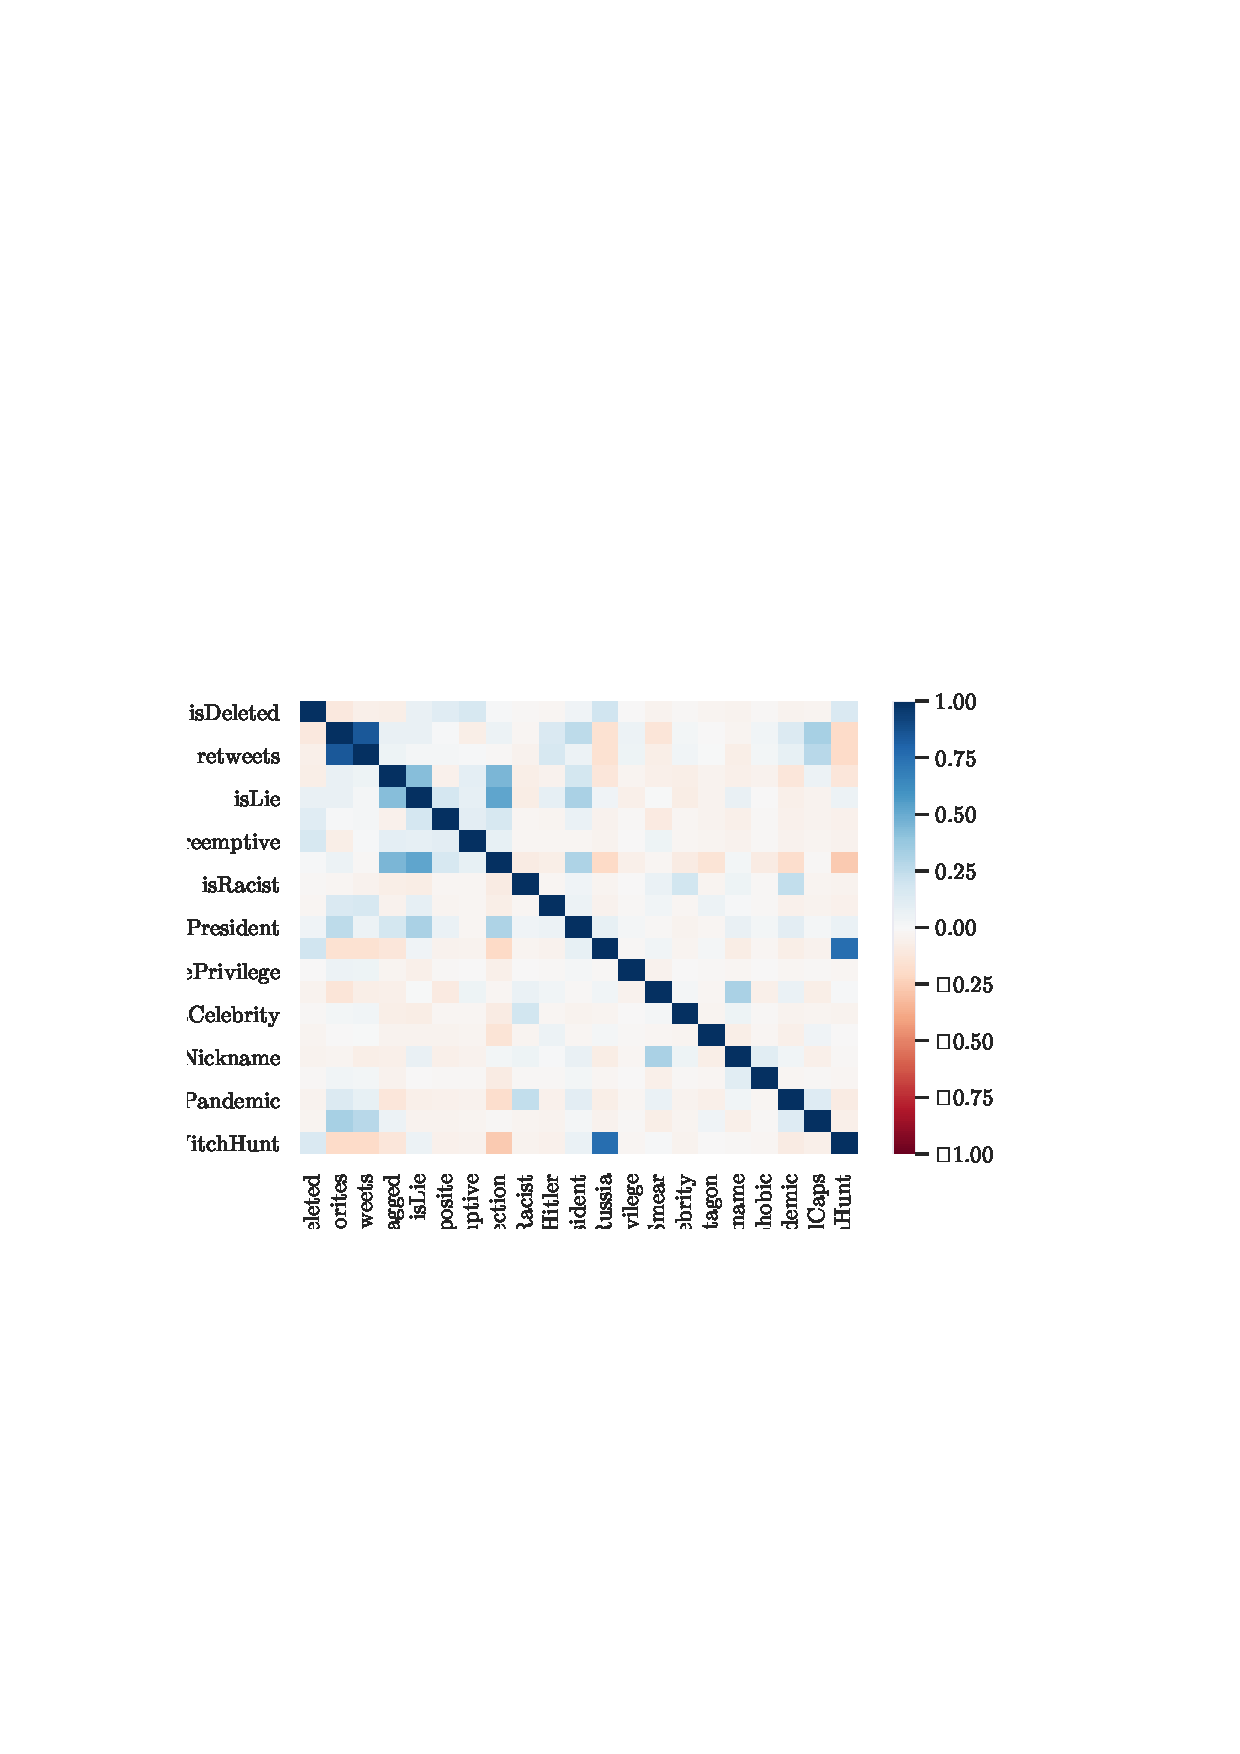
\includegraphics[scale=.8]{corr_heatmap.pdf}
         \caption{Matrix visualization of Pearson\'s correlation coefficient.}
    \end{figure}
    

\end{document}